\documentclass[14pt]{extbook}
\usepackage{multicol, enumerate, enumitem, hyperref, color, soul, setspace, parskip, fancyhdr} %General Packages
\usepackage{amssymb, amsthm, amsmath, latexsym, units, mathtools} %Math Packages
\everymath{\displaystyle} %All math in Display Style
% Packages with additional options
\usepackage[headsep=0.5cm,headheight=12pt, left=1 in,right= 1 in,top= 1 in,bottom= 1 in]{geometry}
\usepackage[usenames,dvipsnames]{xcolor}
\usepackage{dashrule}  % Package to use the command below to create lines between items
\newcommand{\litem}[1]{\item#1\hspace*{-1cm}\rule{\textwidth}{0.4pt}}
\pagestyle{fancy}
\lhead{Makeup Progress Quiz 2}
\chead{}
\rhead{Version B}
\lfoot{5763-3522}
\cfoot{}
\rfoot{Spring 2021}
\begin{document}

\begin{enumerate}
\litem{
Graph the equation below.\[ f(x) = -(x+4)^2 + 19 \]\begin{enumerate}[label=\Alph*.]
\begin{multicols}{2}\item 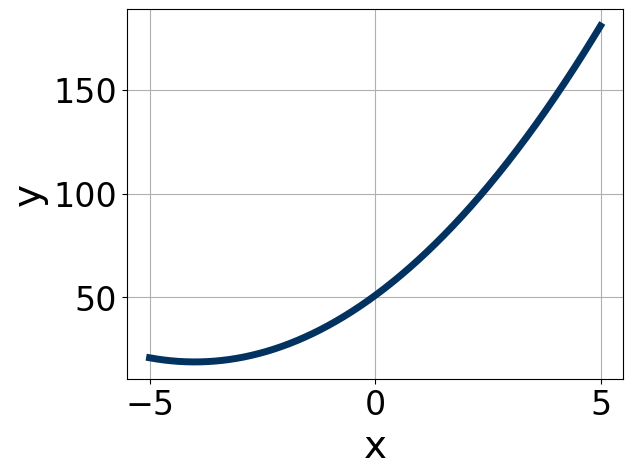
\includegraphics[width = 0.3\textwidth]{../Figures/quadraticEquationToGraphAB.png}\item 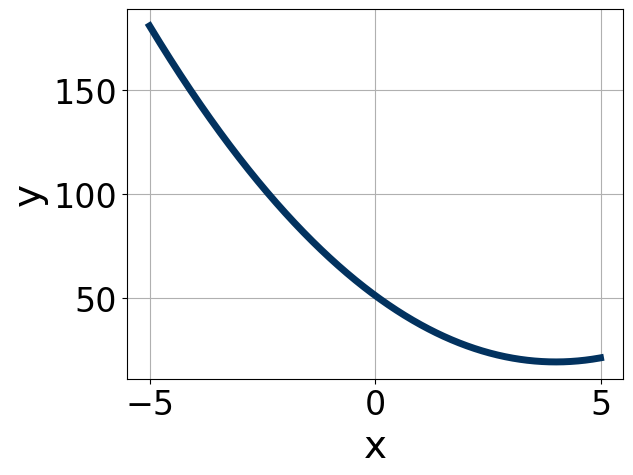
\includegraphics[width = 0.3\textwidth]{../Figures/quadraticEquationToGraphBB.png}\item 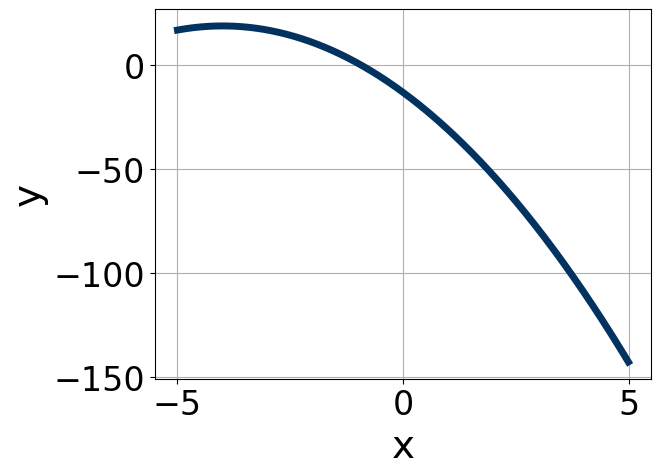
\includegraphics[width = 0.3\textwidth]{../Figures/quadraticEquationToGraphCB.png}\item 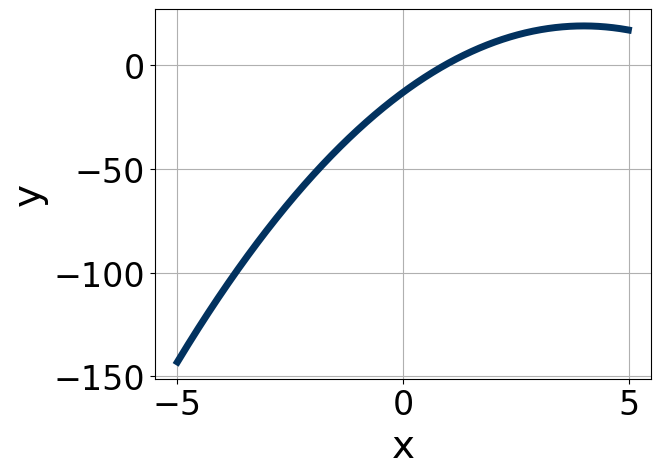
\includegraphics[width = 0.3\textwidth]{../Figures/quadraticEquationToGraphDB.png}\end{multicols}\item None of the above.
\end{enumerate} }
\litem{
Write the equation of the graph presented below in the form $f(x)=ax^2+bx+c$, assuming  $a=1$ or $a=-1$. Then, choose the intervals that $a, b,$ and $c$ belong to.
\begin{center}
    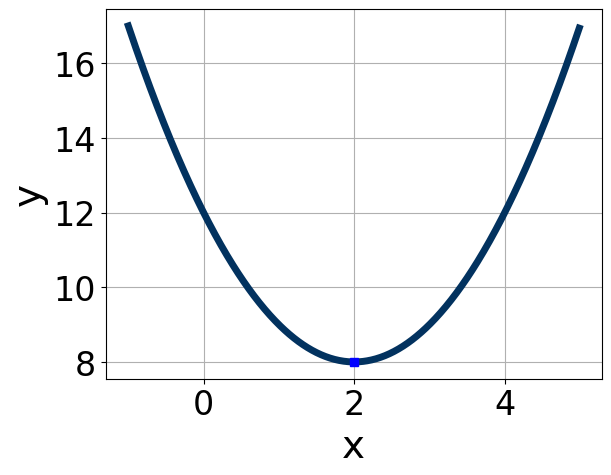
\includegraphics[width=0.5\textwidth]{../Figures/quadraticGraphToEquationB.png}
\end{center}
\begin{enumerate}[label=\Alph*.]
\item \( a \in [0.4, 1.4], \hspace*{5mm} b \in [3, 7], \text{ and } \hspace*{5mm} c \in [-4, 0] \)
\item \( a \in [0.4, 1.4], \hspace*{5mm} b \in [-4, -3], \text{ and } \hspace*{5mm} c \in [10, 15] \)
\item \( a \in [-2.4, -0.5], \hspace*{5mm} b \in [3, 7], \text{ and } \hspace*{5mm} c \in [3, 5] \)
\item \( a \in [-2.4, -0.5], \hspace*{5mm} b \in [-4, -3], \text{ and } \hspace*{5mm} c \in [3, 5] \)
\item \( a \in [0.4, 1.4], \hspace*{5mm} b \in [3, 7], \text{ and } \hspace*{5mm} c \in [10, 15] \)

\end{enumerate} }
\litem{
Solve the quadratic equation below. Then, choose the intervals that the solutions $x_1$ and $x_2$ belong to, with $x_1 \leq x_2$.\[ 15x^{2} -38 x + 24 = 0 \]\begin{enumerate}[label=\Alph*.]
\item \( x_1 \in [0.53, 0.65] \text{ and } x_2 \in [2.38, 3.12] \)
\item \( x_1 \in [1.17, 1.24] \text{ and } x_2 \in [0.83, 1.86] \)
\item \( x_1 \in [0.41, 0.47] \text{ and } x_2 \in [3.51, 3.96] \)
\item \( x_1 \in [17.97, 18] \text{ and } x_2 \in [19.68, 20.6] \)
\item \( x_1 \in [0.39, 0.42] \text{ and } x_2 \in [3.76, 4.43] \)

\end{enumerate} }
\litem{
Solve the quadratic equation below. Then, choose the intervals that the solutions belong to, with $x_1 \leq x_2$ (if they exist).\[ -12x^{2} +15 x + 2 = 0 \]\begin{enumerate}[label=\Alph*.]
\item \( x_1 \in [-17.82, -16.82] \text{ and } x_2 \in [18.44, 18.62] \)
\item \( x_1 \in [-2, -1.36] \text{ and } x_2 \in [0, 0.19] \)
\item \( x_1 \in [-16.64, -16.01] \text{ and } x_2 \in [1.39, 1.46] \)
\item \( x_1 \in [-0.74, 0.04] \text{ and } x_2 \in [1.27, 1.39] \)
\item \( \text{There are no Real solutions.} \)

\end{enumerate} }
\litem{
Graph the equation below.\[ f(x) = (x+3)^2 + 14 \]\begin{enumerate}[label=\Alph*.]
\begin{multicols}{2}\item 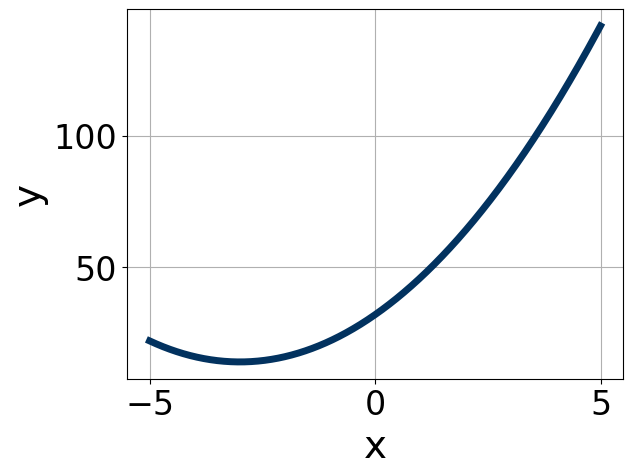
\includegraphics[width = 0.3\textwidth]{../Figures/quadraticEquationToGraphCopyAB.png}\item 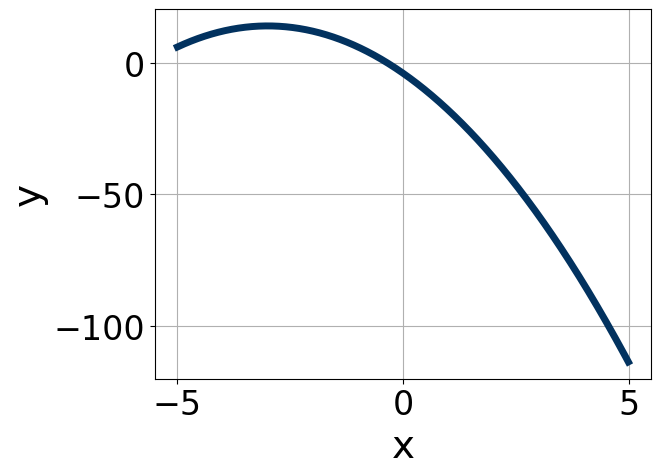
\includegraphics[width = 0.3\textwidth]{../Figures/quadraticEquationToGraphCopyBB.png}\item 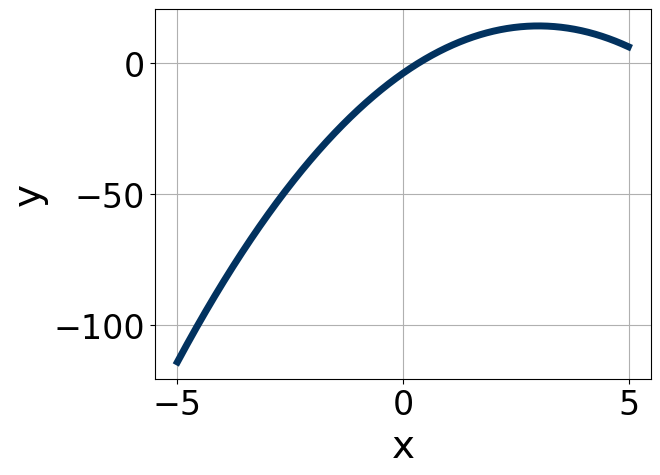
\includegraphics[width = 0.3\textwidth]{../Figures/quadraticEquationToGraphCopyCB.png}\item 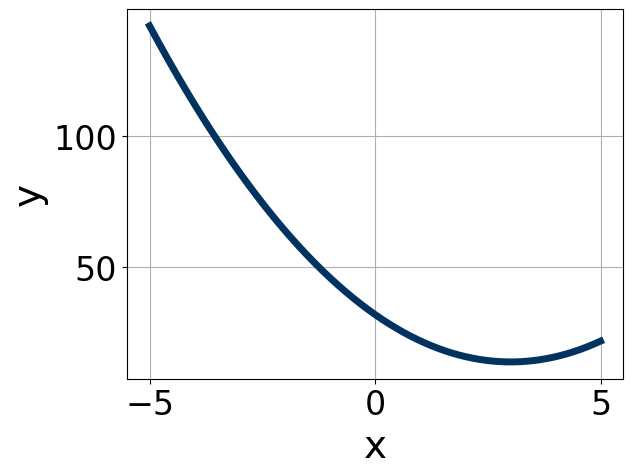
\includegraphics[width = 0.3\textwidth]{../Figures/quadraticEquationToGraphCopyDB.png}\end{multicols}\item None of the above.
\end{enumerate} }
\litem{
Factor the quadratic below. Then, choose the intervals that contain the constants in the form $(ax+b)(cx+d); b \leq d.$\[ 54x^{2} -21 x -20 \]\begin{enumerate}[label=\Alph*.]
\item \( a \in [0.3, 1.9], \hspace*{5mm} b \in [-46, -39], \hspace*{5mm} c \in [0, 2], \text{ and } \hspace*{5mm} d \in [23, 27] \)
\item \( a \in [17.5, 20.3], \hspace*{5mm} b \in [-5, -1], \hspace*{5mm} c \in [2, 5], \text{ and } \hspace*{5mm} d \in [-1, 5] \)
\item \( a \in [4.3, 7.8], \hspace*{5mm} b \in [-5, -1], \hspace*{5mm} c \in [9, 13], \text{ and } \hspace*{5mm} d \in [-1, 5] \)
\item \( a \in [1.9, 5.2], \hspace*{5mm} b \in [-5, -1], \hspace*{5mm} c \in [26, 30], \text{ and } \hspace*{5mm} d \in [-1, 5] \)
\item \( \text{None of the above.} \)

\end{enumerate} }
\litem{
Write the equation of the graph presented below in the form $f(x)=ax^2+bx+c$, assuming  $a=1$ or $a=-1$. Then, choose the intervals that $a, b,$ and $c$ belong to.
\begin{center}
    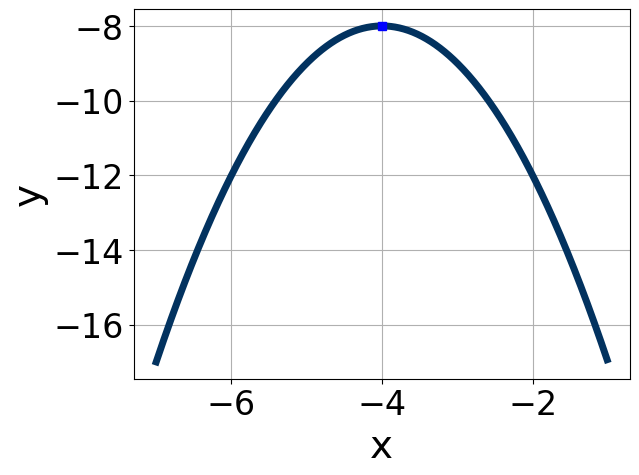
\includegraphics[width=0.5\textwidth]{../Figures/quadraticGraphToEquationCopyB.png}
\end{center}
\begin{enumerate}[label=\Alph*.]
\item \( a \in [-0.4, 1.6], \hspace*{5mm} b \in [6, 11], \text{ and } \hspace*{5mm} c \in [8, 9] \)
\item \( a \in [-0.4, 1.6], \hspace*{5mm} b \in [-11, -7], \text{ and } \hspace*{5mm} c \in [8, 9] \)
\item \( a \in [-1.4, -0.2], \hspace*{5mm} b \in [6, 11], \text{ and } \hspace*{5mm} c \in [-9, -5] \)
\item \( a \in [-1.4, -0.2], \hspace*{5mm} b \in [-11, -7], \text{ and } \hspace*{5mm} c \in [-24, -22] \)
\item \( a \in [-1.4, -0.2], \hspace*{5mm} b \in [6, 11], \text{ and } \hspace*{5mm} c \in [-24, -22] \)

\end{enumerate} }
\litem{
Factor the quadratic below. Then, choose the intervals that contain the constants in the form $(ax+b)(cx+d); b \leq d.$\[ 54x^{2} -57 x + 10 \]\begin{enumerate}[label=\Alph*.]
\item \( a \in [1.76, 2.33], \hspace*{5mm} b \in [-8, -4], \hspace*{5mm} c \in [25.2, 30.1], \text{ and } \hspace*{5mm} d \in [-7, 0] \)
\item \( a \in [5.32, 6.83], \hspace*{5mm} b \in [-8, -4], \hspace*{5mm} c \in [6.1, 12.9], \text{ and } \hspace*{5mm} d \in [-7, 0] \)
\item \( a \in [0.95, 1.95], \hspace*{5mm} b \in [-46, -41], \hspace*{5mm} c \in [-1, 2.2], \text{ and } \hspace*{5mm} d \in [-17, -9] \)
\item \( a \in [17.37, 18.54], \hspace*{5mm} b \in [-8, -4], \hspace*{5mm} c \in [1.9, 6.4], \text{ and } \hspace*{5mm} d \in [-7, 0] \)
\item \( \text{None of the above.} \)

\end{enumerate} }
\litem{
Solve the quadratic equation below. Then, choose the intervals that the solutions belong to, with $x_1 \leq x_2$ (if they exist).\[ 16x^{2} -12 x -7 = 0 \]\begin{enumerate}[label=\Alph*.]
\item \( x_1 \in [-7.4, -4.7] \text{ and } x_2 \in [17.54, 18.33] \)
\item \( x_1 \in [-3, -0.7] \text{ and } x_2 \in [0.25, 0.78] \)
\item \( x_1 \in [-24.3, -23.3] \text{ and } x_2 \in [24.64, 25.09] \)
\item \( x_1 \in [-0.8, 0.6] \text{ and } x_2 \in [0.98, 1.38] \)
\item \( \text{There are no Real solutions.} \)

\end{enumerate} }
\litem{
Solve the quadratic equation below. Then, choose the intervals that the solutions $x_1$ and $x_2$ belong to, with $x_1 \leq x_2$.\[ 15x^{2} -8 x -16 = 0 \]\begin{enumerate}[label=\Alph*.]
\item \( x_1 \in [-2.89, -1.54] \text{ and } x_2 \in [0.51, 0.68] \)
\item \( x_1 \in [-4.62, -2.99] \text{ and } x_2 \in [0.05, 0.36] \)
\item \( x_1 \in [-1.26, -0.74] \text{ and } x_2 \in [1.03, 1.62] \)
\item \( x_1 \in [-13.02, -10.78] \text{ and } x_2 \in [19.62, 20.68] \)
\item \( x_1 \in [-0.69, 1.18] \text{ and } x_2 \in [2.37, 2.9] \)

\end{enumerate} }
\end{enumerate}

\end{document}